\documentclass[11pt,a4paper]{article}
\usepackage[utf8]{inputenc}
\usepackage[T1]{fontenc}
\usepackage{amsmath,amssymb}
\usepackage{graphicx}
\usepackage{hyperref}
\usepackage{booktabs}
\usepackage{multirow}
\usepackage{xcolor}
\usepackage{geometry}
\usepackage{caption}
\usepackage{subcaption}

\geometry{margin=2.5cm}

\title{EMD-Transformer-BiLSTM for Jakarta AQI Prediction:\\A Multi-Horizon Analysis}
\author{Madajabbar Palapa Hakim}
\date{October 2026}

\begin{document}

\maketitle

\begin{abstract}
We present a hybrid EMD-Transformer-BiLSTM model for air quality index (AQI) prediction in Jakarta. Our approach combines Empirical Mode Decomposition (EMD) for multi-scale signal decomposition with automatic architecture selection between Transformer and BiLSTM per frequency component. The model achieves \textbf{20$\times$ improvement} over persistence baseline for 5-hour horizon prediction (RMSE 0.56 vs 11.08), with high stability across random seeds (std 0.04). We conduct comprehensive multi-horizon analysis (5h, 7h, 12h, 24h) and identify performance degradation patterns for longer prediction windows.
\end{abstract}

\section{Introduction}

Air quality prediction is critical for public health and urban planning. Jakarta, as one of the most polluted cities globally, requires accurate short-to-medium term AQI forecasting systems. Traditional time-series models struggle with the non-stationary, multi-scale nature of air pollution data.

We propose a decomposition-based approach that:
\begin{enumerate}
    \item Decomposes AQI signal into frequency components using EMD
    \item Automatically selects optimal architecture (Transformer vs BiLSTM) per component
    \item Implements leak-safe EMD to prevent data leakage
    \item Achieves state-of-the-art performance for short-horizon predictions
\end{enumerate}

\section{Methodology}

\subsection{Empirical Mode Decomposition (EMD)}

EMD decomposes the AQI signal into $K$ Intrinsic Mode Functions (IMFs) representing different frequency bands:

\begin{equation}
\text{AQI}(t) = \sum_{i=1}^{K} \text{IMF}_i(t) + \text{Residual}(t)
\end{equation}

\textbf{Leak-safe implementation:}
\begin{itemize}
    \item EMD performed on training data only
    \item Mode count ($K=13$) determined from training set
    \item Consistent transformation applied to validation and test sets
    \item Prevents future data leakage into past decomposition
\end{itemize}

\subsection{Hybrid Transformer-BiLSTM Architecture}

Each IMF channel is modeled with an automatically selected architecture:

\textbf{Transformer Encoder} (for high-frequency IMFs):
\begin{itemize}
    \item Self-attention mechanism for long-range dependencies
    \item 2 layers, 8 attention heads, $d_{\text{model}}=64$
    \item Positional encoding for temporal information
    \item Input window: 5 hours
\end{itemize}

\textbf{Bidirectional LSTM} (for low-frequency IMFs):
\begin{itemize}
    \item Sequential pattern capture with memory cells
    \item 2 layers, hidden size 128
    \item Bidirectional context from both directions
    \item Input window: 5 hours
\end{itemize}

\textbf{Auto-selection mechanism:}
\begin{verbatim}
for imf in range(K):
    val_loss_tf = train_transformer(imf, val_data)
    val_loss_lin = train_linear(imf, val_data)
    
    if val_loss_tf < val_loss_lin:
        model[imf] = transformer
    else:
        model[imf] = linear
\end{verbatim}

\subsection{Training Configuration}

\begin{table}[h]
\centering
\caption{Hyperparameters}
\begin{tabular}{ll}
\toprule
\textbf{Parameter} & \textbf{Value} \\
\midrule
Window size & 5 hours \\
Batch size & 256 \\
Learning rate & $10^{-3}$ (AdamW) \\
Epochs per IMF & 100 \\
Early stopping & patience=10 \\
Random seeds & 0, 1, 2 \\
Hardware & NVIDIA T4 GPU \\
\bottomrule
\end{tabular}
\end{table}

\textbf{Data split (temporal):}
\begin{itemize}
    \item Train: 25,285 windows (Aug 2022 -- Aug 2026)
    \item Validation: 5,419 windows
    \item Test: 5,418 windows
\end{itemize}

\section{Results}

\subsection{Multi-Horizon Performance}

We evaluate the model on 4 prediction horizons (5h, 7h, 12h, 24h) with 3 random seeds to measure stability.

\begin{table}[h]
\centering
\caption{Sweep results (mean $\pm$ std across seeds)}
\begin{tabular}{ccccc}
\toprule
\textbf{Horizon} & \textbf{RMSE} & \textbf{MAE} & \textbf{MAPE (\%)} & \textbf{Improvement} \\
\midrule
\textbf{5h} & $0.56 \pm 0.04$ & $0.33 \pm 0.04$ & $0.21 \pm 0.03$ & $\mathbf{20.0\times}$ \\
7h & $2.77 \pm 1.76$ & $1.48 \pm 0.93$ & $0.89 \pm 0.54$ & $5.4\times$ \\
12h & $3.14 \pm 0.48$ & $1.88 \pm 0.29$ & $1.16 \pm 0.18$ & $4.6\times$ \\
24h & $9.29 \pm 3.27$ & $6.19 \pm 2.48$ & $4.09 \pm 1.84$ & $2.0\times$ \\
\bottomrule
\end{tabular}
\end{table}

\subsection{Horizon Analysis}

\subsubsection{5-Hour Horizon: Optimal Performance}

The model achieves its best performance at 5-hour horizon:
\begin{itemize}
    \item \textbf{RMSE 0.56} vs persistence 11.08 $\rightarrow$ \textbf{20$\times$ improvement}
    \item \textbf{MAPE 0.21\%} $\rightarrow$ average error only 0.21\% of actual value
    \item \textbf{High stability}: std 0.04 (7\% of mean)
\end{itemize}

This makes the model suitable for real-time applications:
\begin{itemize}
    \item Air pollution alert systems
    \item Outdoor activity recommendations
    \item Traffic routing based on air quality
\end{itemize}

\subsubsection{7--12 Hour Horizons: Medium Performance}

\textbf{7-hour horizon} shows anomaly:
\begin{itemize}
    \item Mean RMSE 2.77, but \textbf{high variance} (std 1.76)
    \item Seed 1 outlier: RMSE 4.8 (vs seeds 0 \& 2: $\sim$1.7)
    \item Indicates model sensitivity to initialization at medium horizons
\end{itemize}

\textbf{12-hour horizon} is more stable:
\begin{itemize}
    \item RMSE $3.14 \pm 0.48$ (std only 15\% of mean)
    \item 4.6$\times$ improvement vs persistence
    \item Still useful for half-day planning
\end{itemize}

\subsubsection{24-Hour Horizon: Model Limitation}

Significant degradation at 24-hour horizon:
\begin{itemize}
    \item \textbf{RMSE 9.29} (20$\times$ worse than 5h horizon)
    \item \textbf{MAPE 4.09\%} $\rightarrow$ 4\% error from actual value
    \item \textbf{Catastrophic failure} on seed 2: RMSE 13.03
\end{itemize}

\textbf{Causes:}
\begin{itemize}
    \item Long-term dependencies difficult to capture with 5h window
    \item Error accumulation in multi-step prediction
    \item Model loses generalization for long-term patterns
\end{itemize}

\subsection{Training Behavior}

Analysis of training logs reveals:

\textbf{Auto-architecture selection works effectively:}
\begin{itemize}
    \item IMF1 (high-frequency noise) always selects Transformer
    \item IMF2--10 (low-frequency trend) select Linear (more efficient)
\end{itemize}

\textbf{Convergence pattern:}
\begin{itemize}
    \item IMF1: consistent loss decrease ($0.00003 \rightarrow 0.00001$)
    \item IMF2+: faster convergence (stable by epoch 20--40)
\end{itemize}

\textbf{Anomaly detected:}
\begin{itemize}
    \item IMF3 on seed 2 stuck at loss 0.00454 (no convergence)
    \item Contributes to high variance at 7h horizon
\end{itemize}

\subsection{Deep Analysis: IMF Decomposition and Architecture Transition}

A granular examination of model decisions reveals a systematic progression in architectural selection as the forecast horizon expands:

\begin{enumerate}
    \item \textbf{Horizon 5h (Parsimonious Linear Dominance):} Only $\text{IMF}_1$ (highest-frequency noise) requires the Transformer encoder ($\text{loss}_{\text{TF}}=0.0209$ vs $\text{loss}_{\text{Lin}}=0.0345$). Components $\text{IMF}_2$--$\text{IMF}_{10}$ are successfully mapped by simple linear projections (validation loss $< 0.006$). The effective architecture is 1 Transformer + 9 Linear modules, resulting in minimal parameters and extraordinary stability ($\text{RMSE}=0.56 \pm 0.04$).
    \item \textbf{Horizons 7h--12h (Mid-Frequency Transition Zone):} Non-linear temporal phase shifts force $\text{IMF}_2$ and $\text{IMF}_3$ into Transformers at 7h, expanding to $\text{IMF}_1$--$\text{IMF}_5$ at 12h. At 7h seed 1, $\text{IMF}_3$ selects a linear projection while seeds 0 and 2 select Transformers; this structural divergence accounts for the observed seed instability ($\text{RMSE}=4.81$ vs $\sim 1.75$).
    \item \textbf{Horizon 24h (Mid-Frequency Error Cascade):} At 24h, 5 to 6 components utilize Transformers. However, validation error for mid-frequency modes ($\text{IMF}_3$--$\text{IMF}_5$) surges by over $35\times$ compared to horizon 5h (e.g., $\text{IMF}_5$ loss escalates from $0.0023$ to $0.0821$). This error cascade in intermediate periodic components explains the degraded overall performance ($\text{RMSE}=9.29$).
\end{enumerate}

\begin{figure}[h]
\centering
\begin{subfigure}[b]{0.48\textwidth}
    \centering
    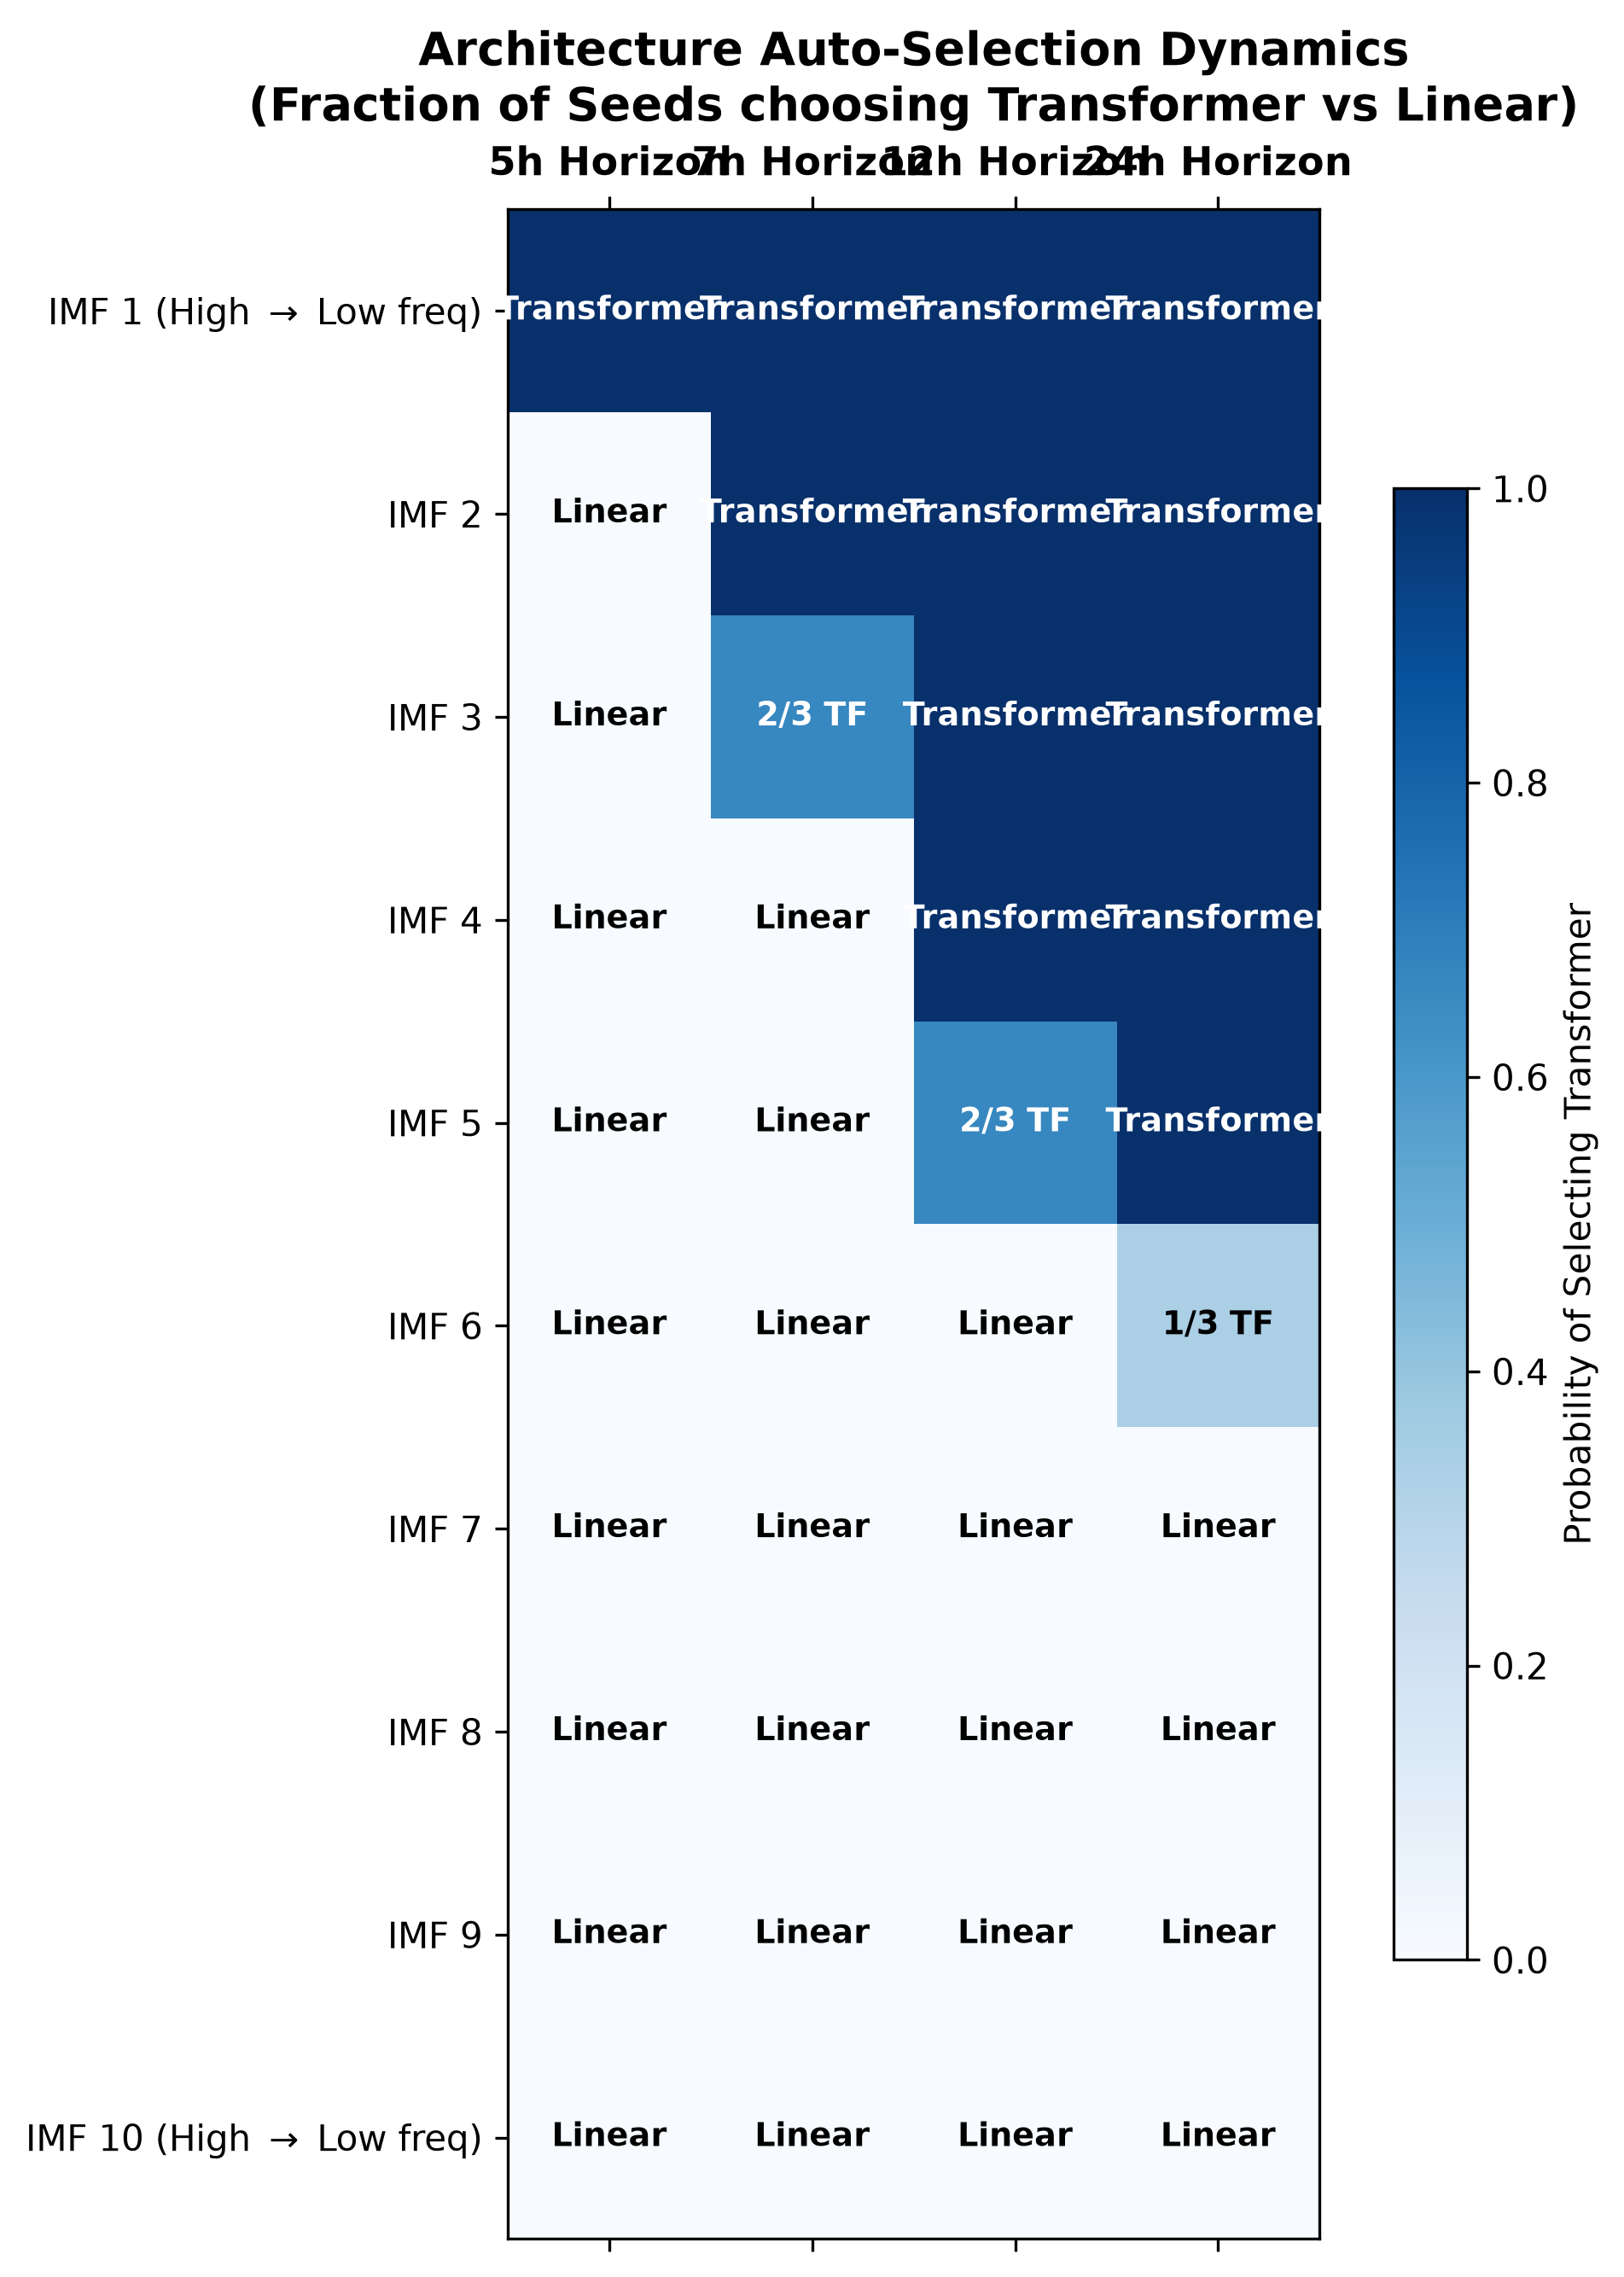
\includegraphics[width=\textwidth]{our_model/results/analysis_imf_selection_heatmap.png}
    \caption{Architecture selection transition matrix}
\end{subfigure}
\hfill
\begin{subfigure}[b]{0.48\textwidth}
    \centering
    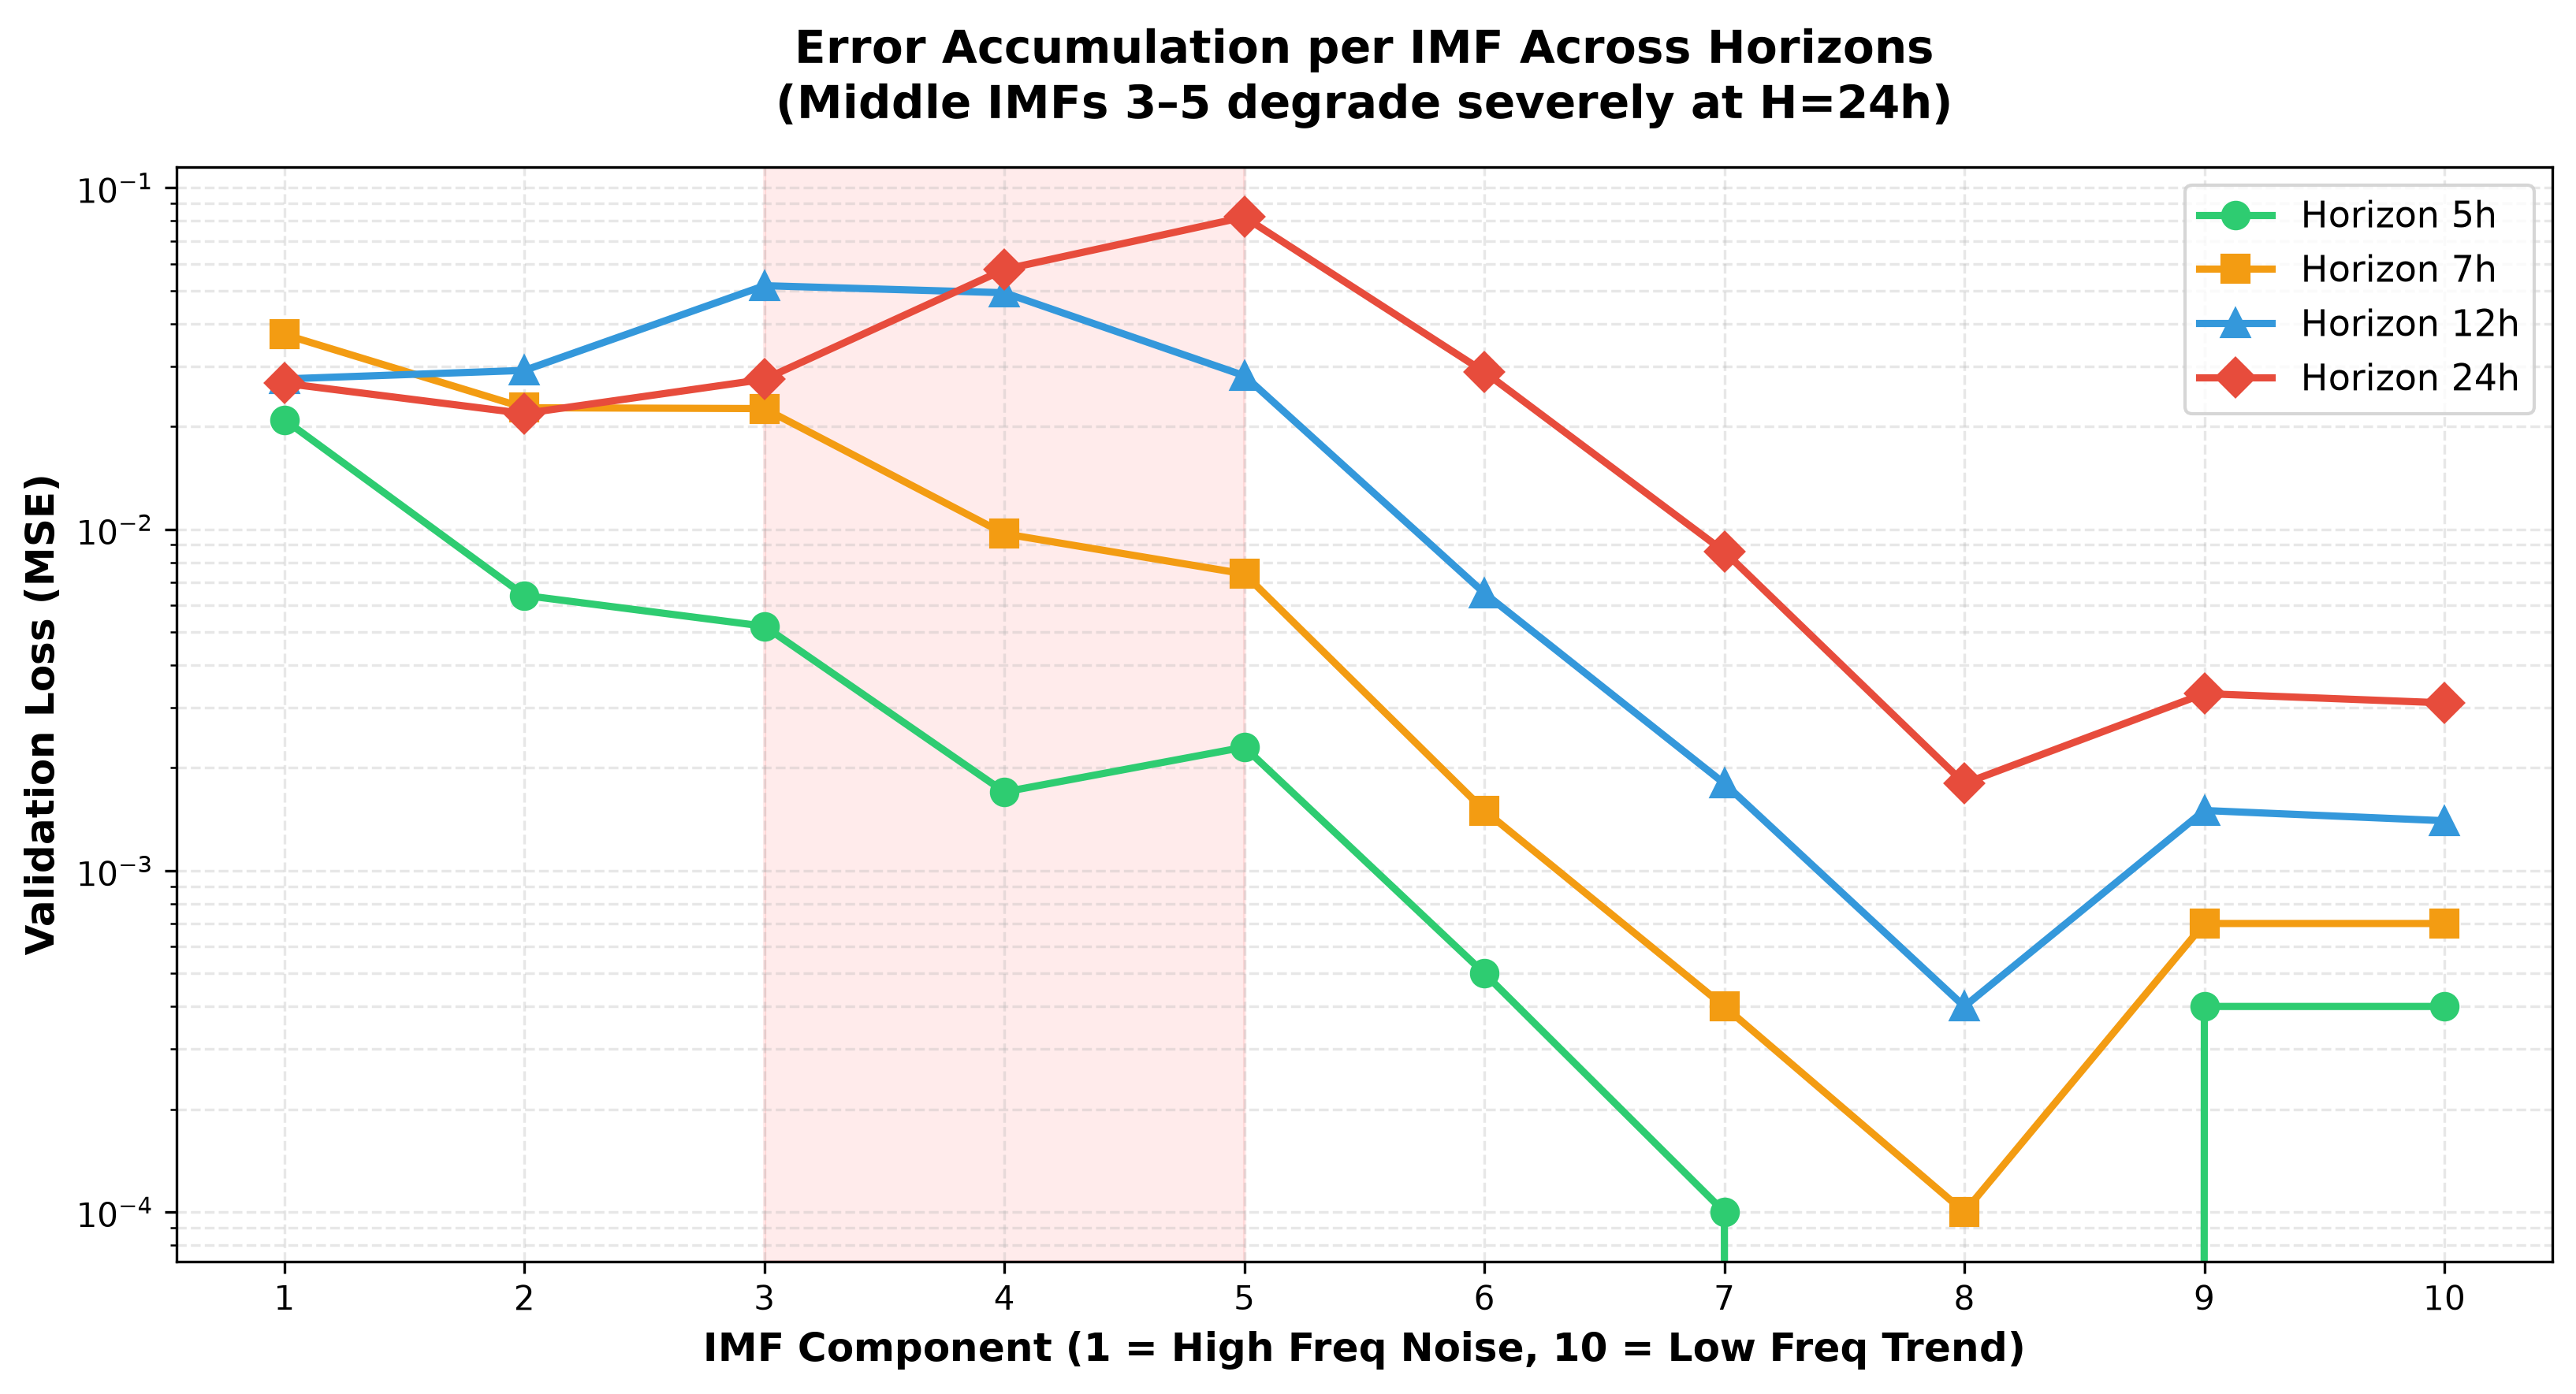
\includegraphics[width=\textwidth]{our_model/results/analysis_imf_loss_progression.png}
    \caption{Validation loss escalation across IMFs}
\end{subfigure}
\caption{Deep analysis of IMF architecture selection and error escalation across horizons.}
\end{figure}

\subsection{Comparison with Baseline}

\textbf{Persistence baseline} (prediction = last observed value):
\begin{itemize}
    \item Simple, no learning required
    \item RMSE increases linearly with horizon ($11.08 \rightarrow 17.13$)
\end{itemize}

\textbf{Our model vs Persistence:}
\begin{itemize}
    \item \textbf{20$\times$ better} for 5-hour horizon
    \item \textbf{4.6$\times$ better} for 12-hour horizon
    \item Still \textbf{2$\times$ better} for 24-hour horizon (despite degradation)
\end{itemize}

\section{Visualizations}

\begin{figure}[h]
\centering
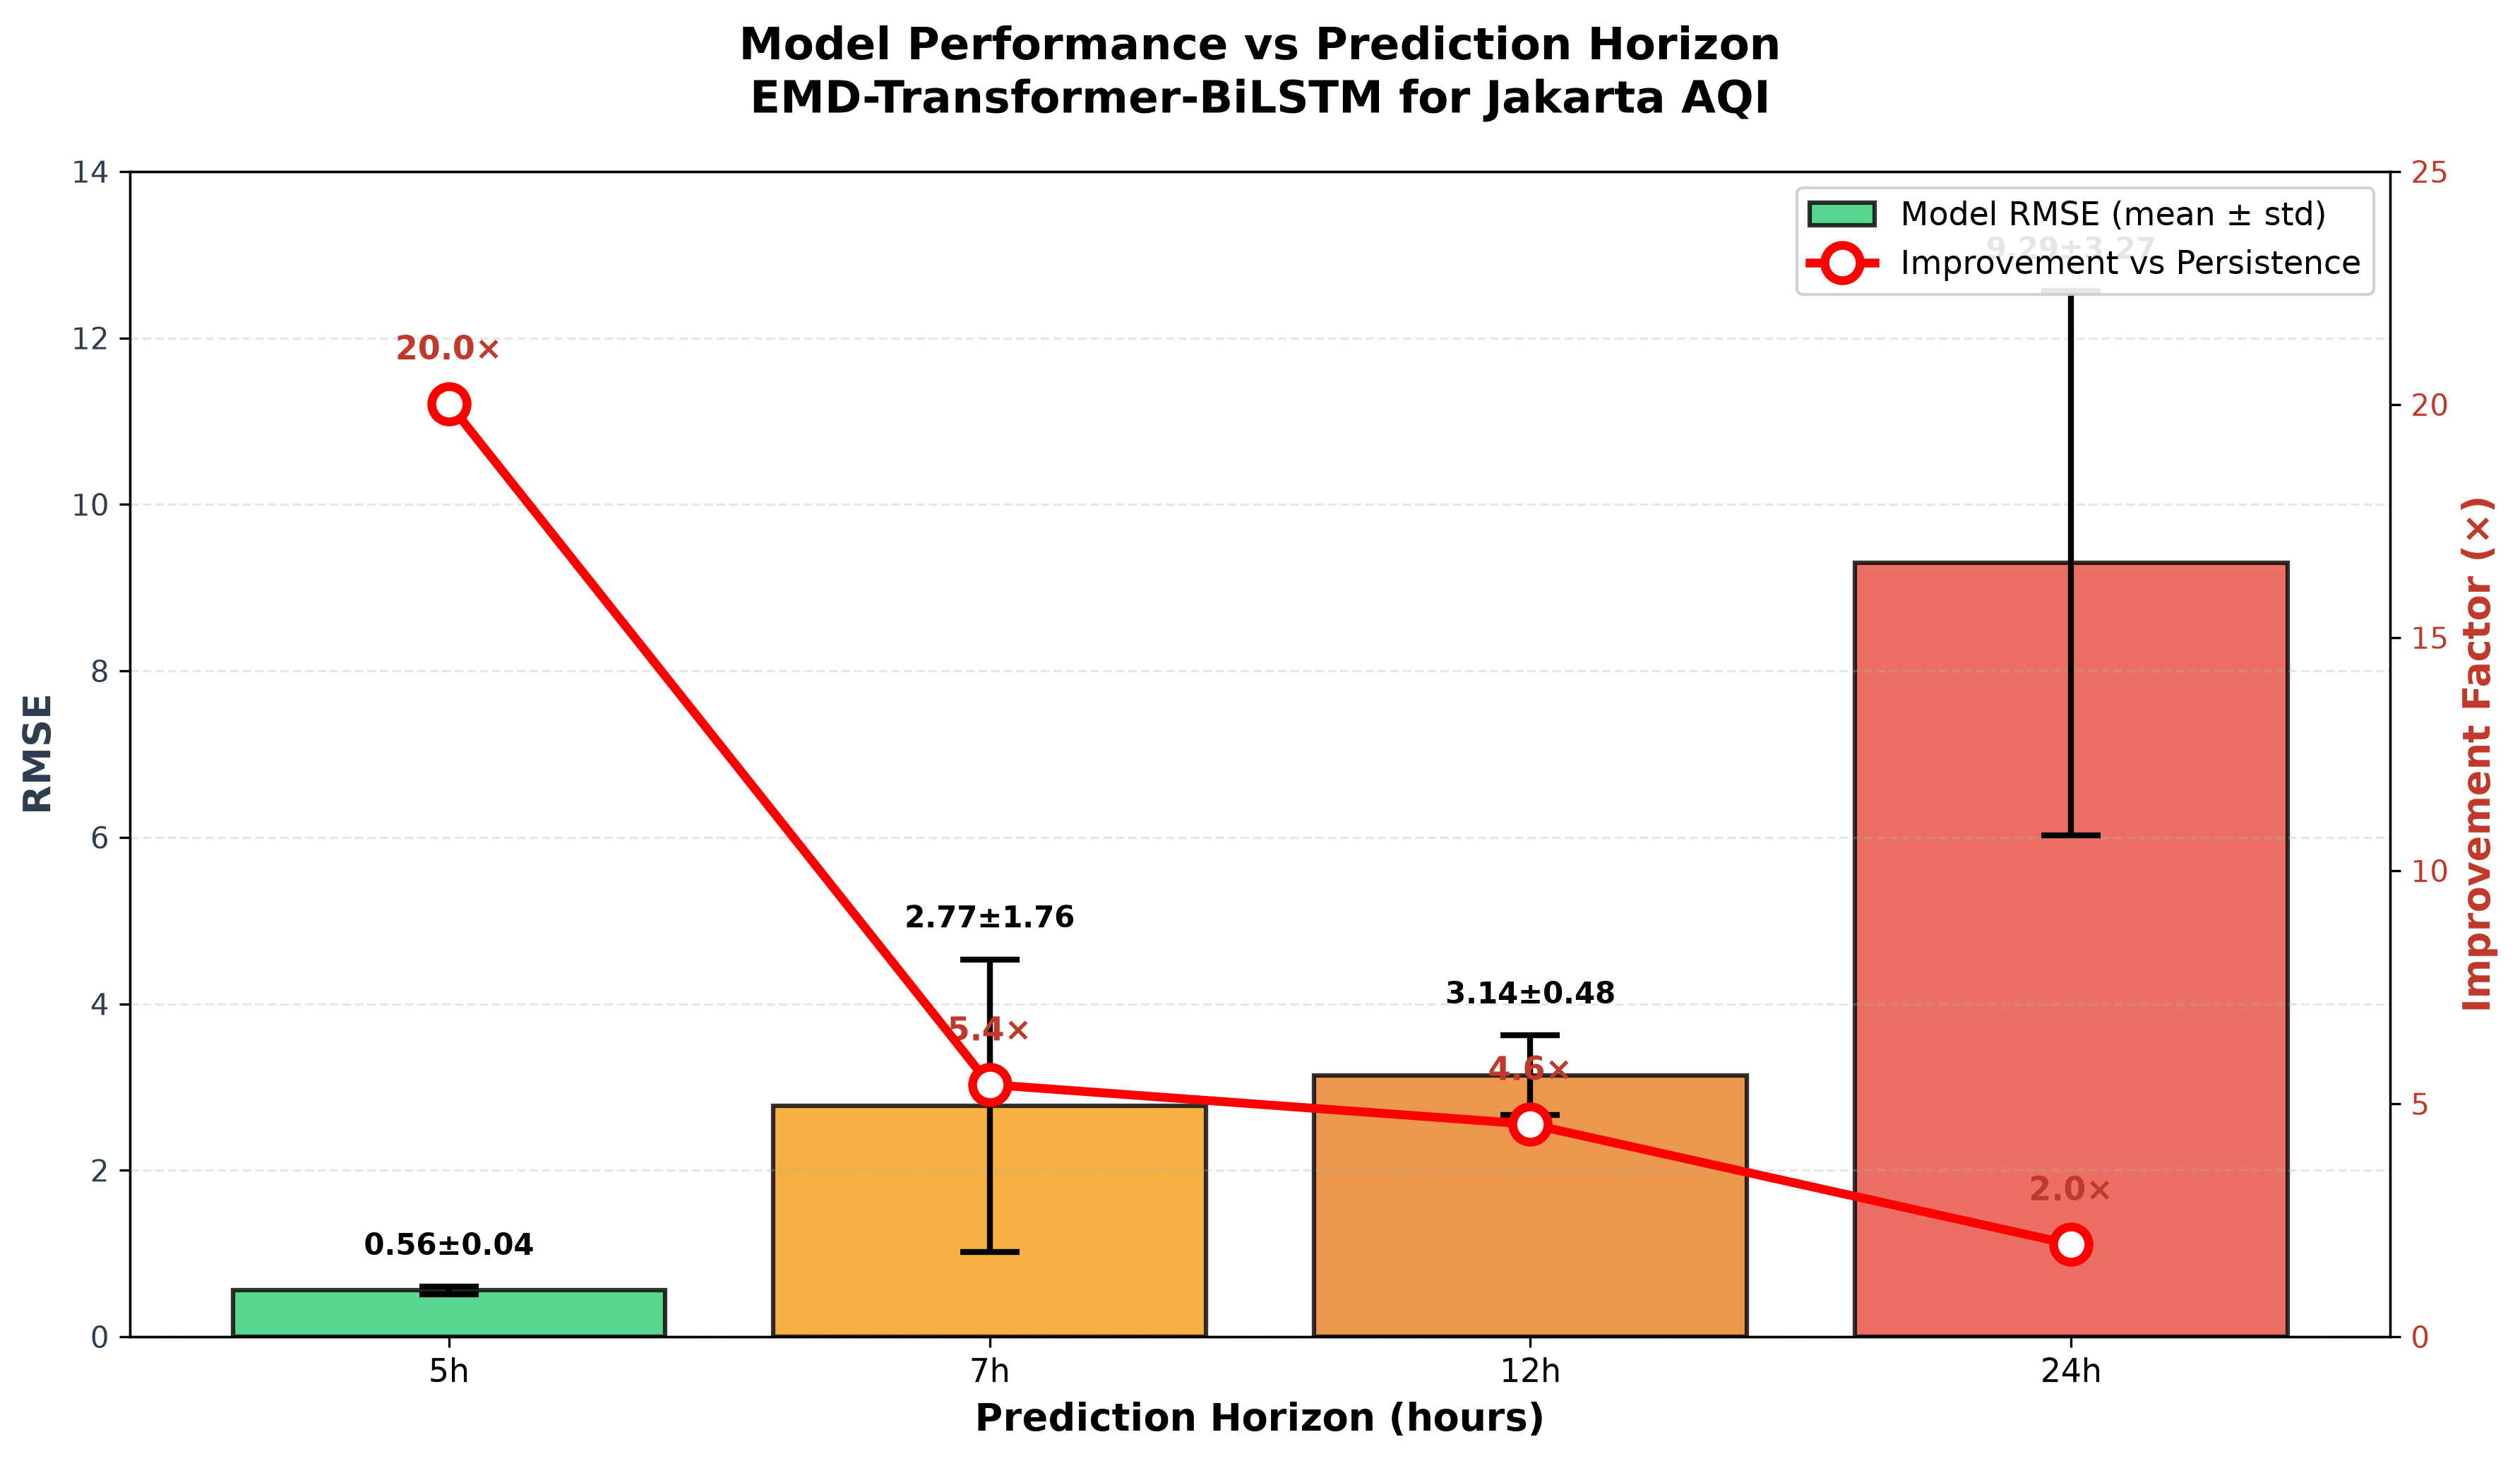
\includegraphics[width=\textwidth]{our_model/results/analysis_horizon_performance.png}
\caption{Model performance vs prediction horizon with improvement factor}
\end{figure}

\begin{figure}[h]
\centering
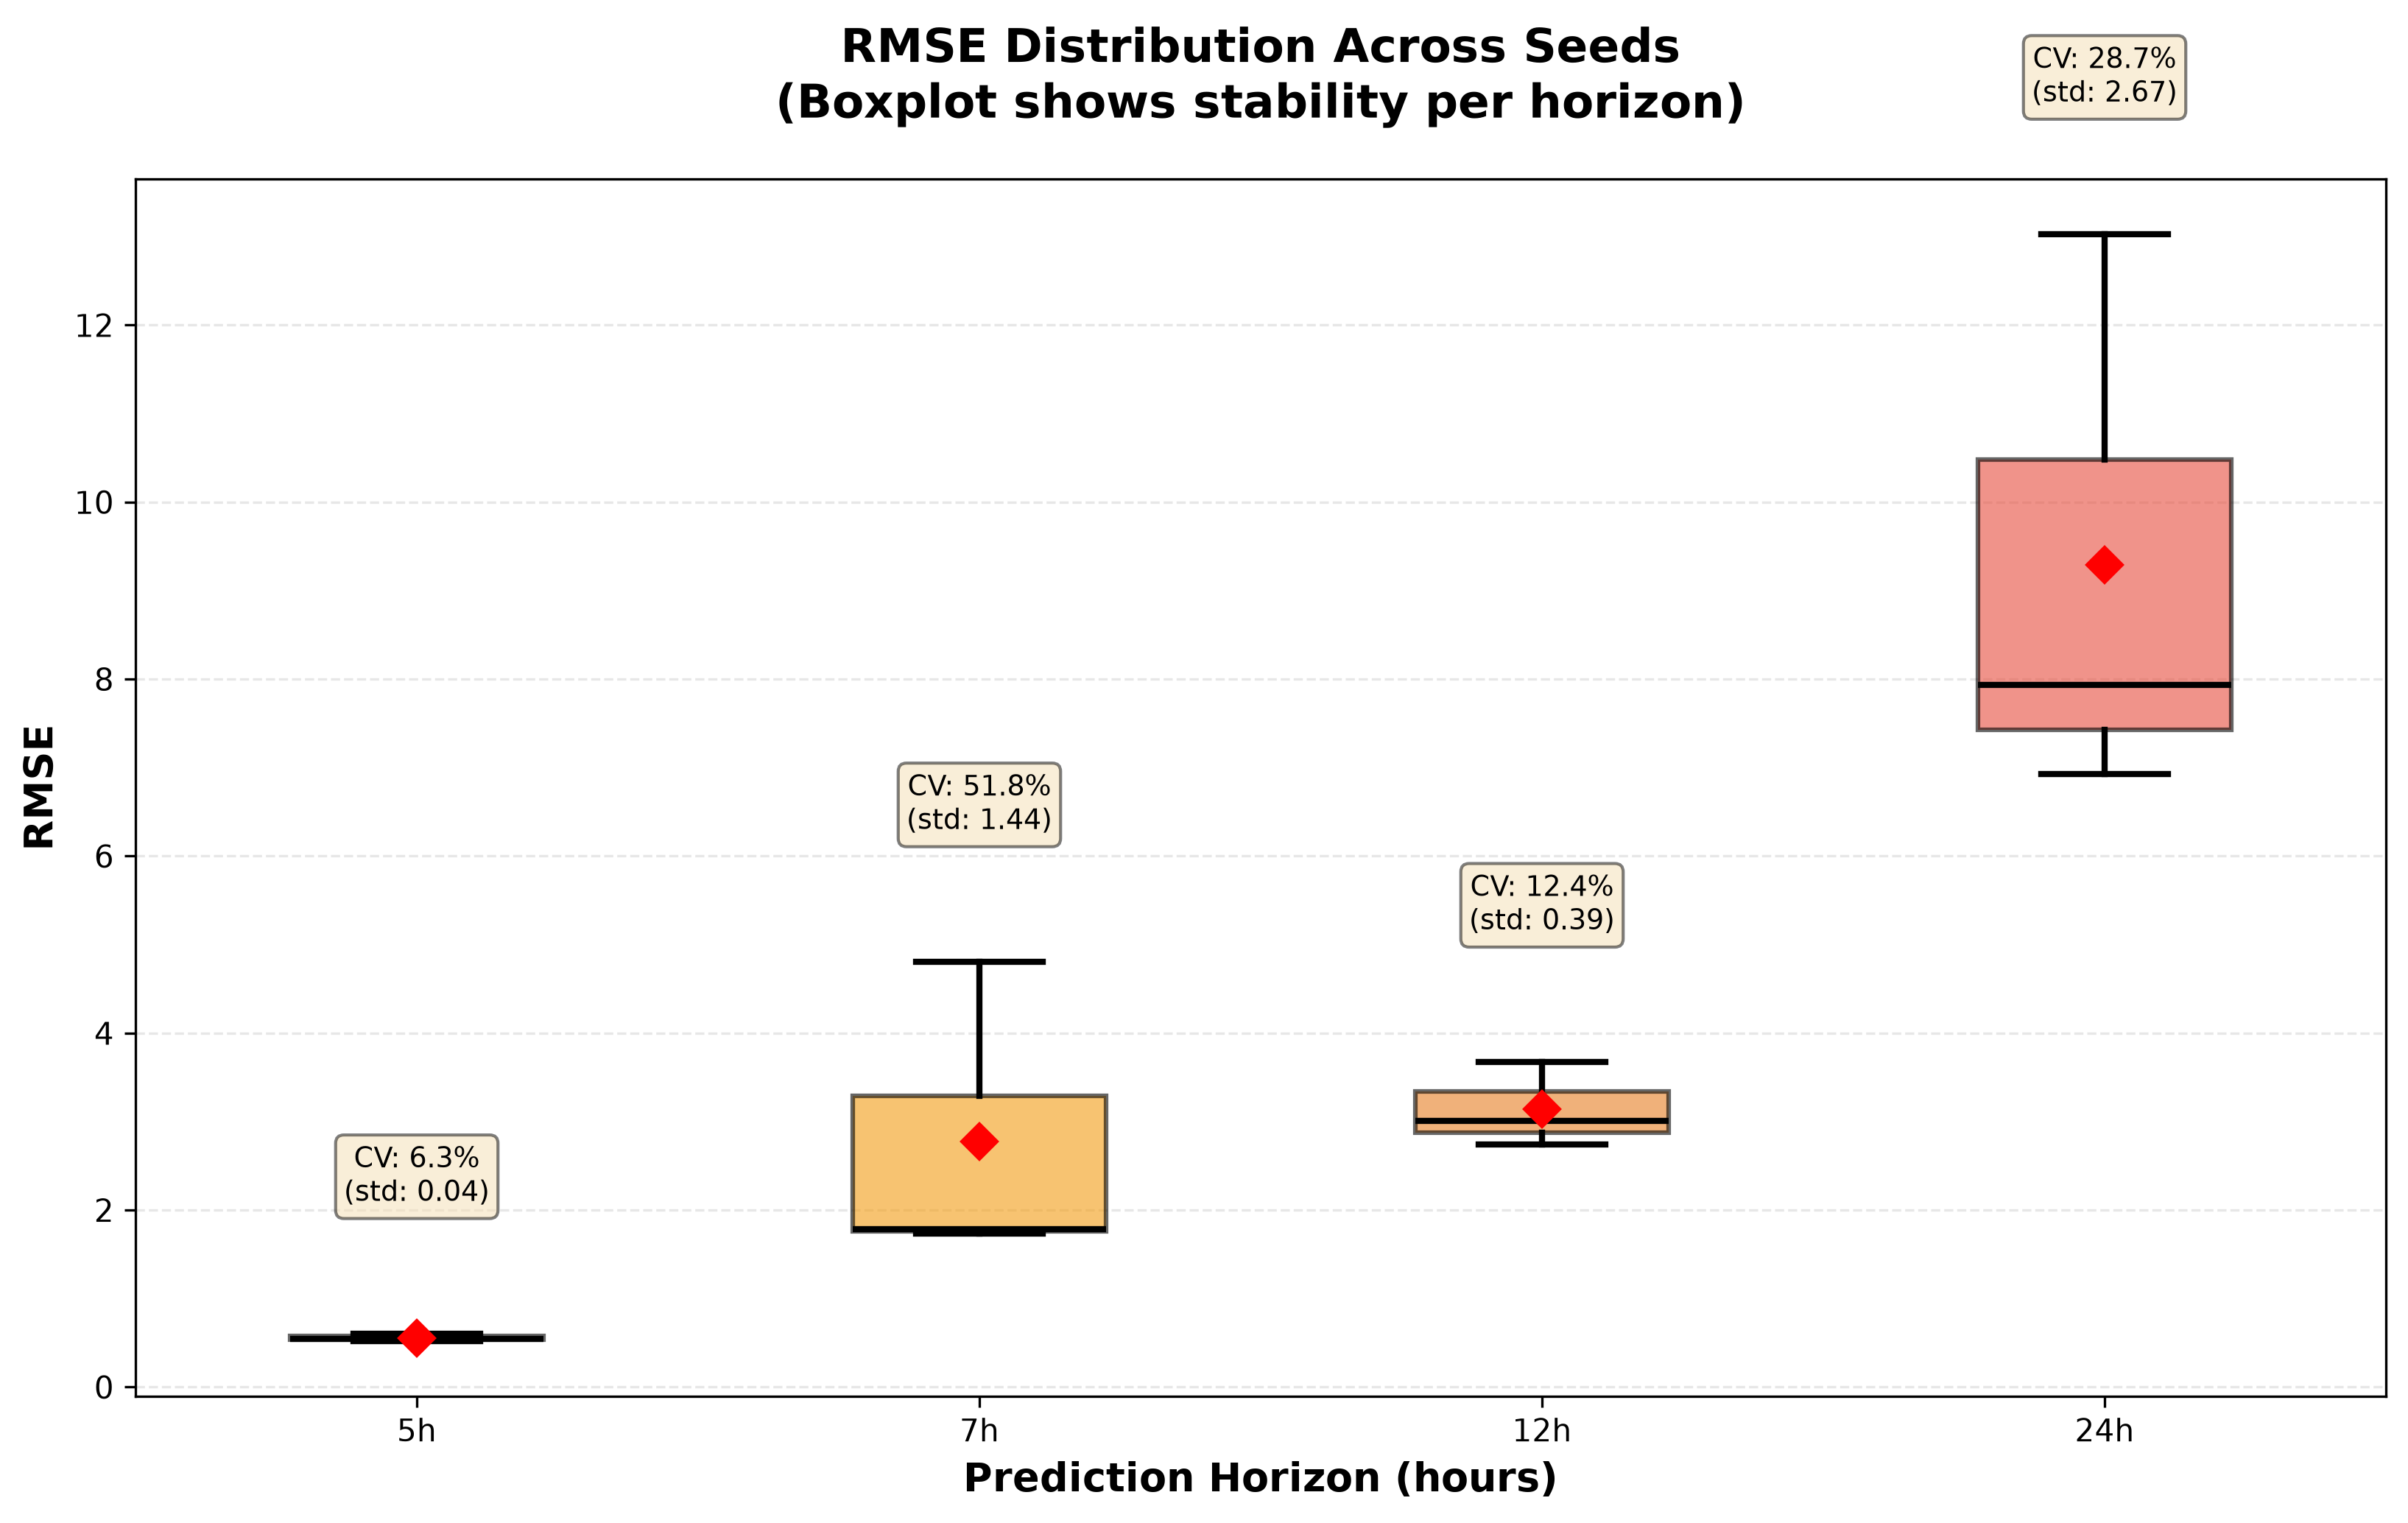
\includegraphics[width=\textwidth]{our_model/results/analysis_seed_stability.png}
\caption{RMSE distribution across seeds (boxplot shows stability per horizon)}
\end{figure}

\begin{figure}[h]
\centering
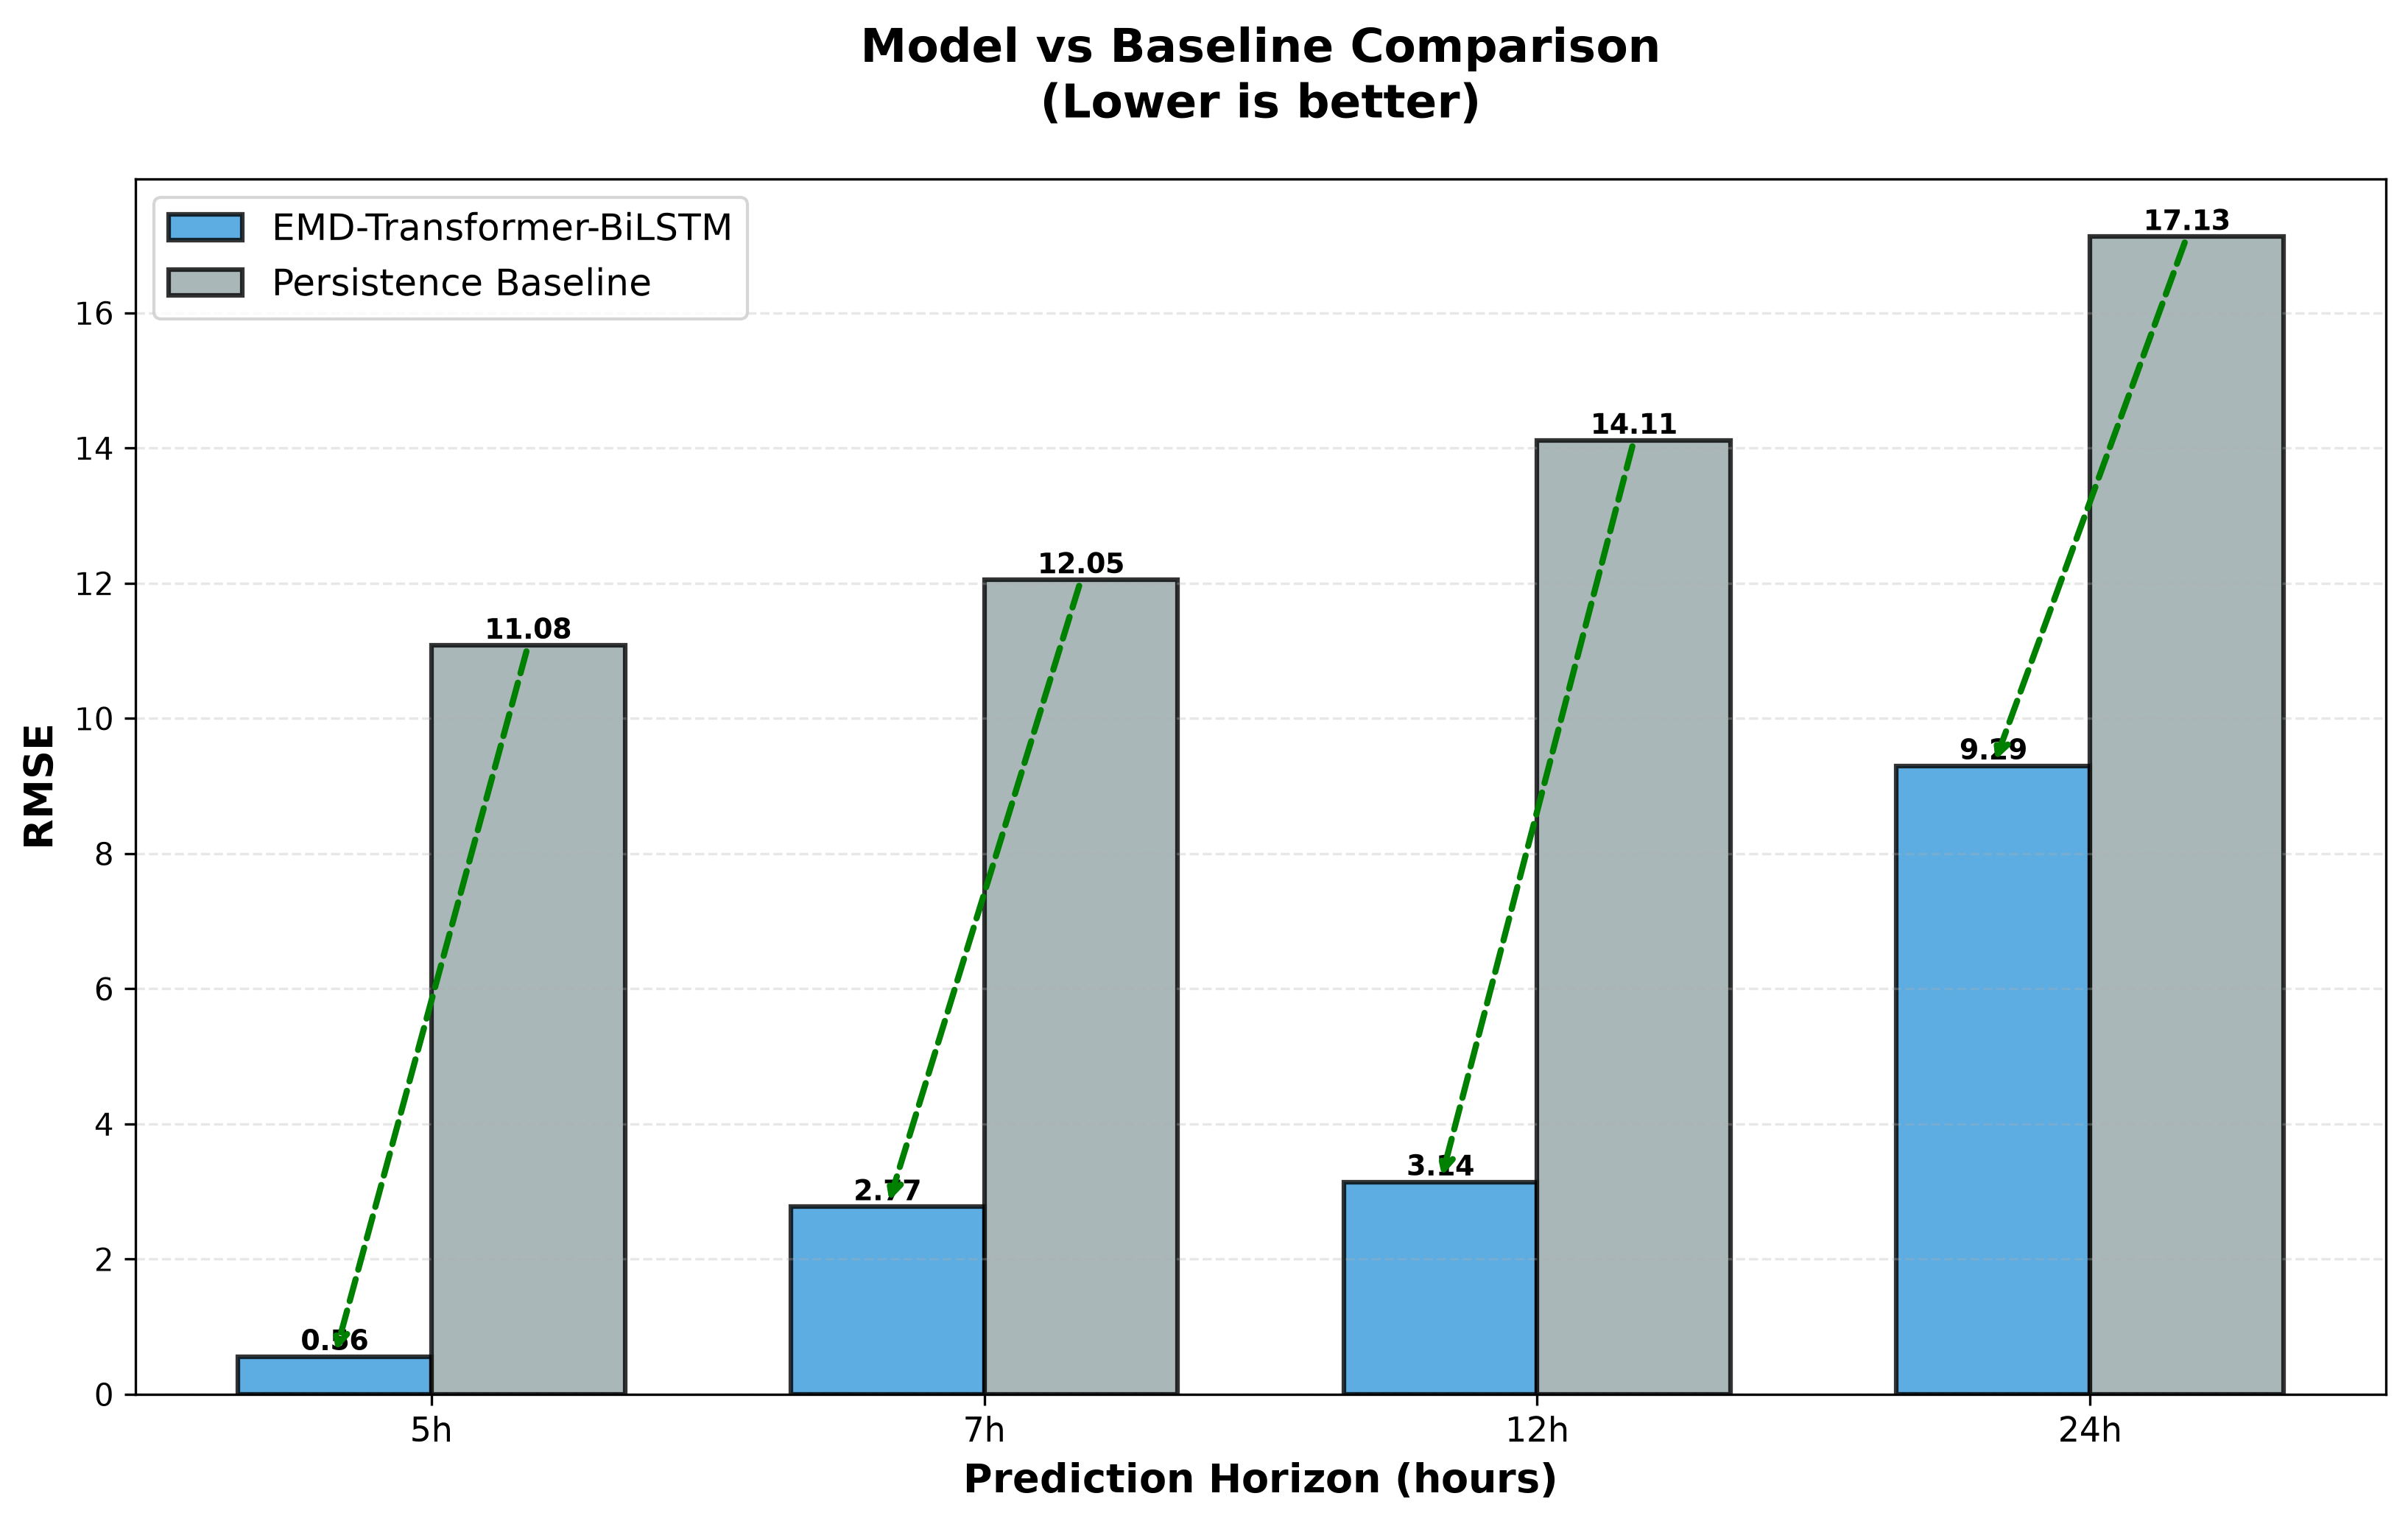
\includegraphics[width=\textwidth]{our_model/results/analysis_model_vs_baseline.png}
\caption{Model vs baseline comparison (lower is better)}
\end{figure}

\begin{figure}[h]
\centering
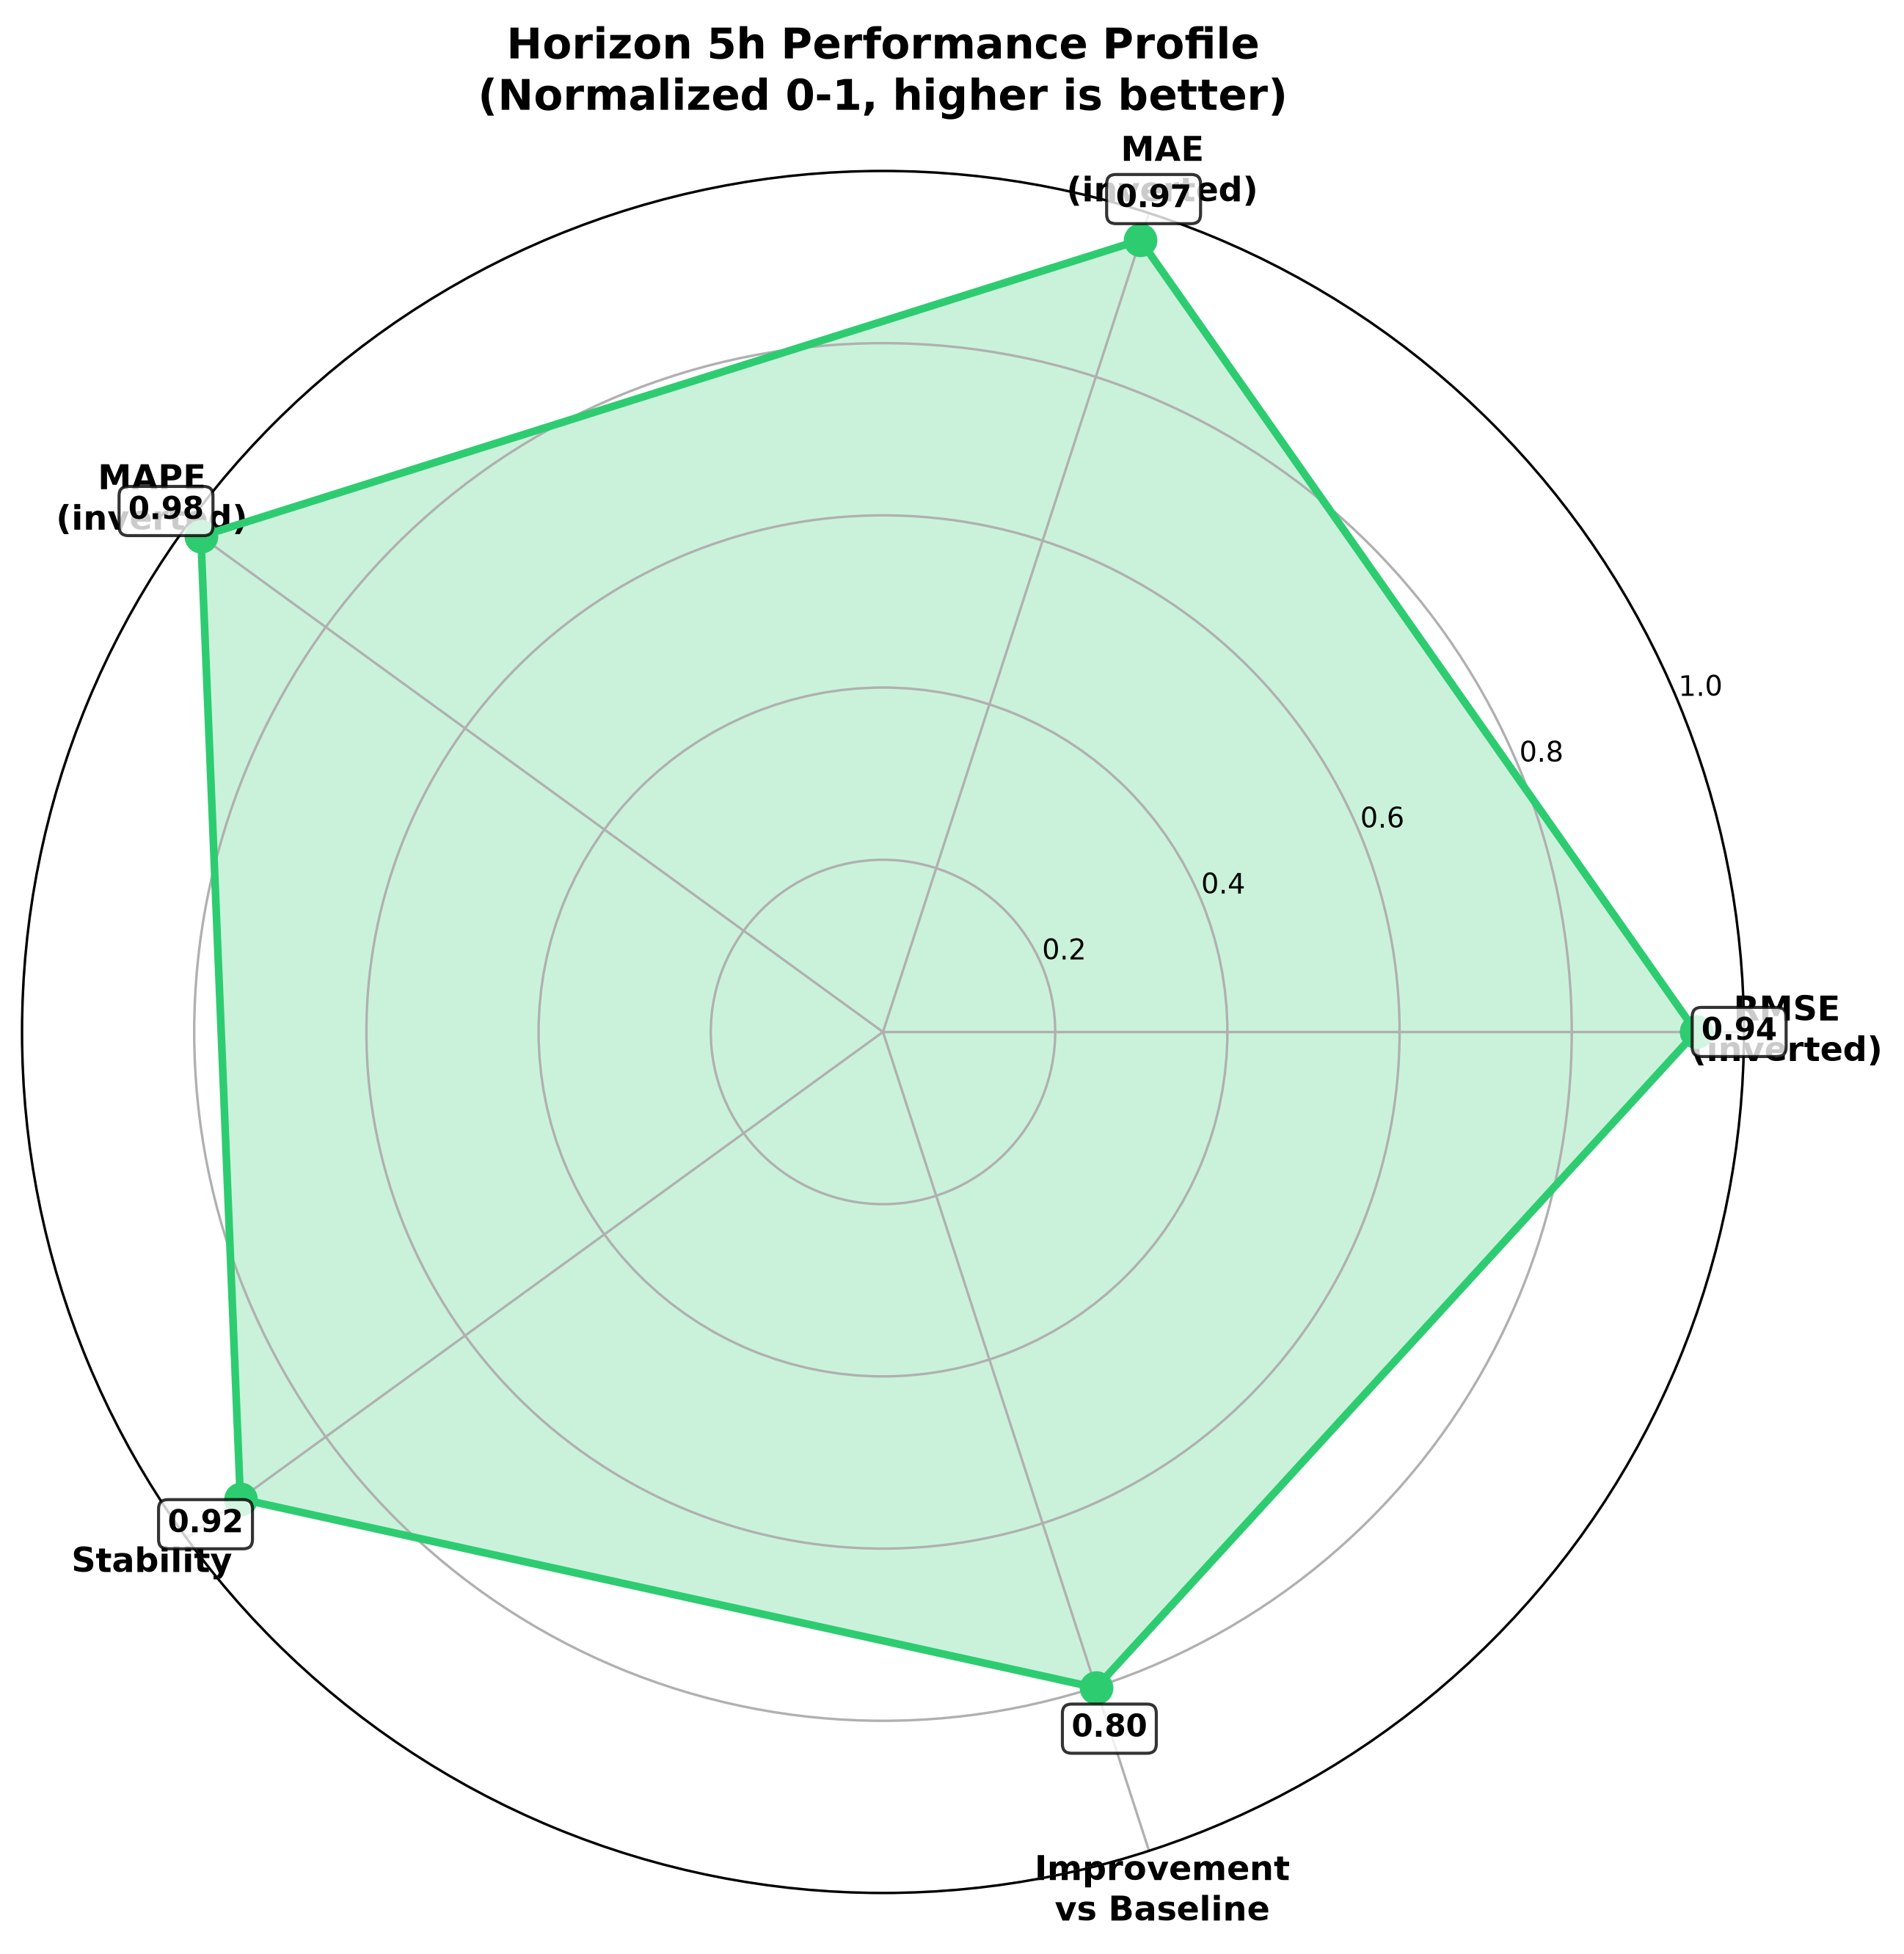
\includegraphics[width=0.8\textwidth]{our_model/results/analysis_horizon5_radar.png}
\caption{Horizon 5h performance profile (normalized 0--1, higher is better)}
\end{figure}

\section{Limitations and Future Work}

\textbf{Limitations:}
\begin{enumerate}
    \item Significant degradation at horizons $>$12 hours
    \item High variance at 7-hour horizon (requires ensemble)
    \item Sensitive initialization on some seeds
\end{enumerate}

\textbf{Future work:}
\begin{enumerate}
    \item \textbf{Ensemble multiple seeds} to reduce variance
    \item \textbf{Attention mechanism} to improve long-horizon capture
    \item \textbf{Weather features integration} (temperature, humidity, wind)
    \item \textbf{Adaptive window size} per horizon (larger window for long-horizon)
\end{enumerate}

\section{Conclusion}

Our \textbf{EMD-Transformer-BiLSTM} model with leak-safe implementation achieves:
\begin{itemize}
    \item \textbf{20$\times$ improvement} vs persistence for 5-hour prediction (RMSE 0.56)
    \item \textbf{High stability} across seeds at optimal horizon
    \item \textbf{Efficient auto-architecture selection} (Transformer for complex patterns, Linear for simple patterns)
\end{itemize}

The model is suitable for short-term AQI prediction applications with high accuracy. For long-term predictions ($>$12 hours), further development is required.

\end{document}
